
\documentclass[10pt, a4paper]{beamer}

\usetheme{Berkeley}
\usecolortheme{sidebartab}

\usepackage{graphicx}
\graphicspath{ {images/} }

\begin{document}
	\setbeamertemplate{sidebar left}{}
	\title{Progress Presentation-I}
	\subtitle{e-Yantra Summer Intership-2017 \\ Modular Robots}
	\author{Srijal Poojari\\Madhav Wagh\\
	\textbf{Mentors}: \\
	 Pushkar Raj, Aditya Panwar and Fayyaz Pocker}
	\institute{IIT, Bombay}
	\date{\today}
	%\addtobeamertemplate{sidebar left}{}{\includegraphics[scale = 0.3]{logowithtext.png}}
	\frame{\titlepage}

\setbeamertemplate{sidebar left}[sidebar theme]
\section{Overview of Project}
\begin{frame}{Overview of Project}
	\begin{itemize}
		\item \textbf{Project Name}:  Modular Robots
		\item \textbf{Objective} 
		\begin{enumerate}
		\item To build a Self-reconfigurable autonomous 	     		robot which can deliberately change shape by 				reorganizing connectivity between the modules.
		\linebreak
		\item To add sensors to the robot and make it smart. 		\\(To sense and take action according to the 				  environment)
		\linebreak
		\end{enumerate}
		\item \textbf{Deliverables}
		\begin{enumerate}
		 \item A stable modular robot which is able to 					  change its shape upon the need of the 					  environment\linebreak
		\item Code and Documentation of each Task (1-6)
		\end{enumerate}
	\end{itemize}
\end{frame}

\section{Overview of Task}
\begin{frame}{Overview of Task}
	\begin{center}
    \begin{tabular}{ | l | p{6cm} | l |}
    \hline
     \textbf{Task No.} & \textbf{Task} & \textbf{Deadline}\\ \hline
     1 & Getting Familiar with existing models of Modular Robots & 2 days  \\ \hline
     
     2 & Interfacing Arduino IDE with Servo, Bluetooth and Sensor & 3 days  \\ \hline
     
     3 & Testing and selecting appropriate sensors to be added in the module & 2 days  \\ \hline
     
     4 & Make design changes in the modules for accommodating sensors.  & 4 days  \\ \hline
      
     5 & Assembling all the selected parts. Four robotic modules need to be produced & 4 days  \\ \hline
     
     6 & Applying algorithm to check different types of motion (Wheel, Snake, Ladder)  & 7 days  \\ \hline
     
     7 & Autonomous Obstacle Avoidance using sensor detection and self-reconfiguration & 6 days  \\ \hline
     
     8 & Code \& Documentation & 6 days  \\ \hline
     
    
    \end{tabular}
\end{center}
	
\end{frame}


\section{Task Accomplised}
\begin{frame}{Task Accomplised}
	\begin{itemize}
		\item \textbf{Task-1: Getting familiar with existing Modular Robots.}
		  \begin{itemize}
		  \item Collected information on existing modular robots.
		  \item Prepared a report and concluded that the Dtto Modular Robot is the most promising option under the given time and resources.
           \end{itemize}
           \vspace{15pt}
        \centering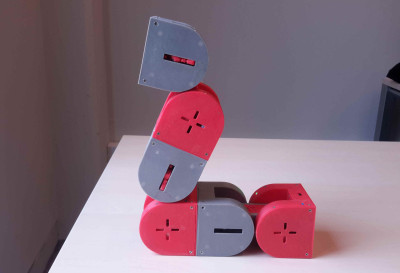
\includegraphics[scale=0.4]{dtto.jpg}   
		
	\end{itemize}
\end{frame}

\section{Task Accomplised}
\begin{frame}{Task Accomplised}
	\begin{itemize}
\item \textbf{Task-2 + 3: Selecting and interfacing sensors, servo motor and Bluetooth module with an Arduino.}
		\begin{itemize}
		  \item Successfully interfaced Bluetooth module HC-05 to HC-05 and HC-05 to PC/Android communication.
		  \item Interfaced servo motors and tested the Sharp IR sensor and VL53L0X ToF sensor for obstacle detection/distance measurement.
           \end{itemize}
           \centering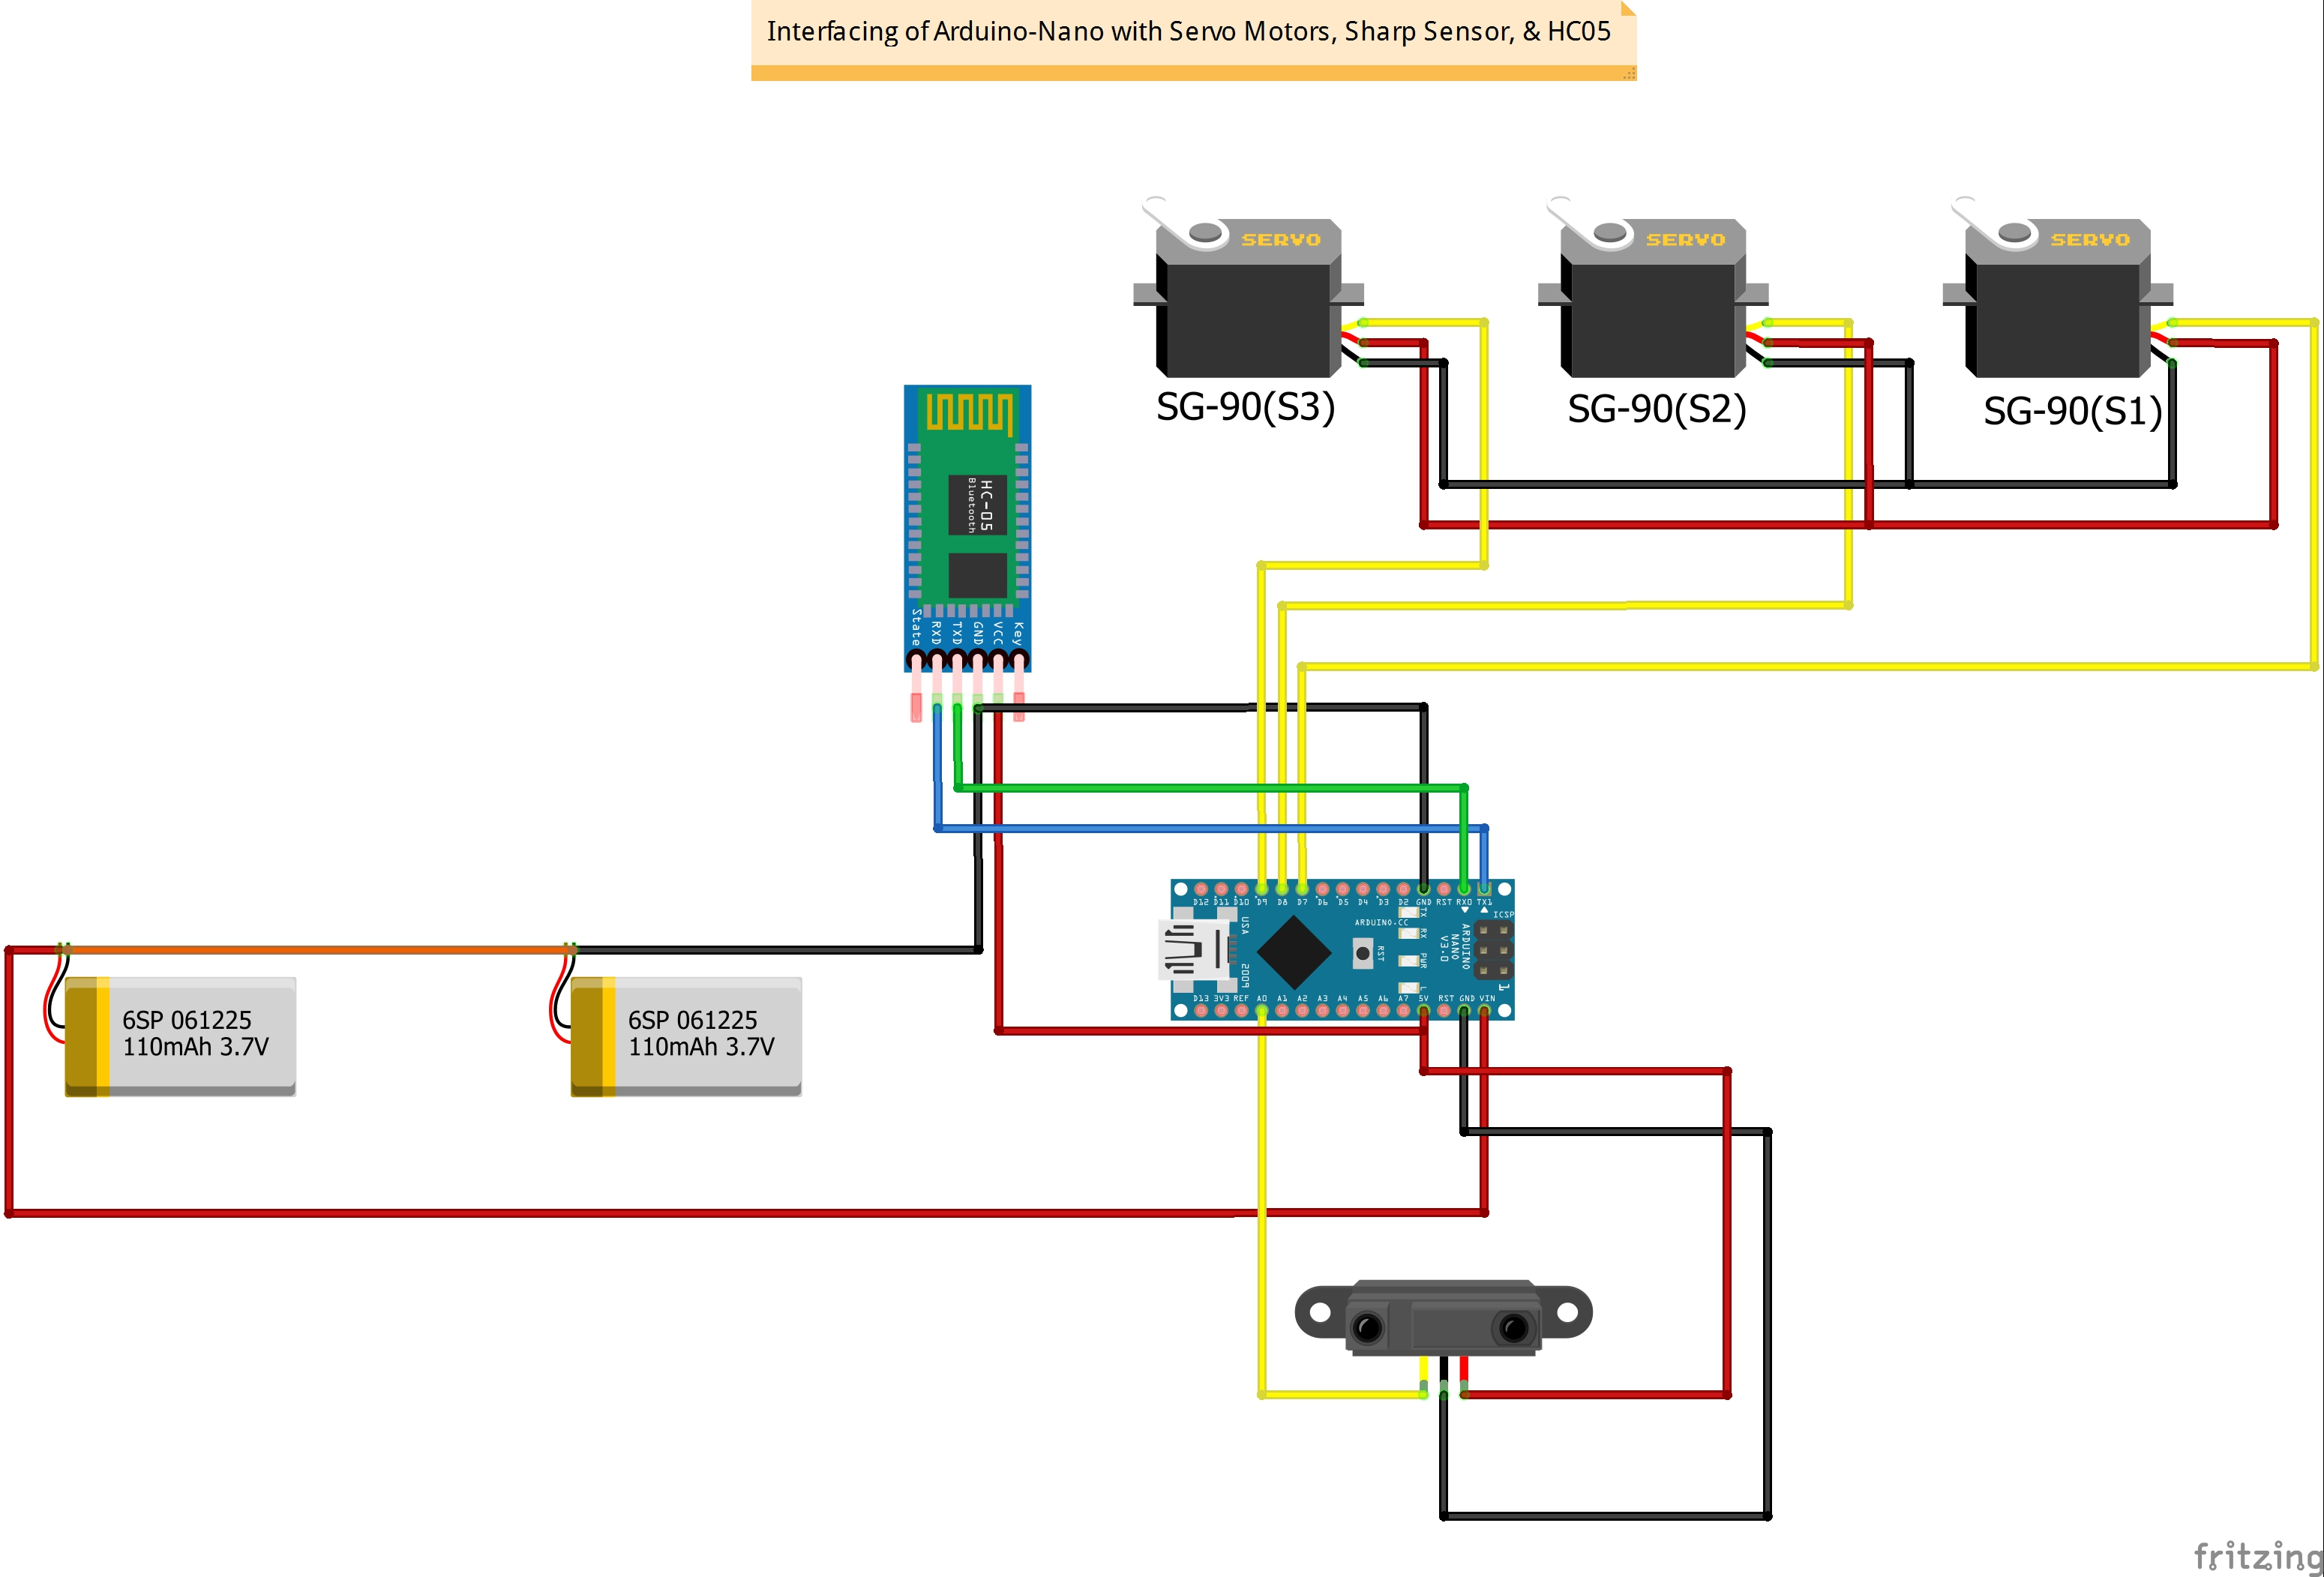
\includegraphics[scale=0.2]{Arduino_interfacing.jpg}
	\end{itemize}
\end{frame}

\section{Task Accomplised}
\begin{frame}{Task Accomplised}
	\begin{itemize}
		\item \textbf{Task-4: Making design changes in the modules.}
		\begin{itemize}
		    \item No major design changes were required as the modules have space for the tiny VL53L0X distance measurement sensor. 
		    \item Holes for the screws had to be expanded due to unavailability of M1.7x4mm screws.
		\end{itemize}
        \centering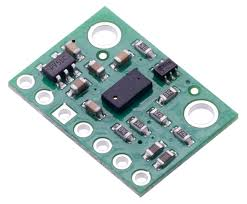
\includegraphics[scale=0.45]{download.jpg}
	\end{itemize}
\end{frame}

\section{Task Accomplised}
\begin{frame}{Task Accomplised}
	\begin{itemize}
		\item \textbf{Simulations in V-REP}
		    \begin{itemize}
		    \item Got familiar with the V-REP environment with Lua scripting and implemented practice simulations.
		    \item Understood existing Dtto movements and modified design to add proximity sensor which can detect obstacles and also measure its height.
		    \item Crossed the detected obstacles by reshaping modules in V-REP. \\ See video.
             \end{itemize}
             \centering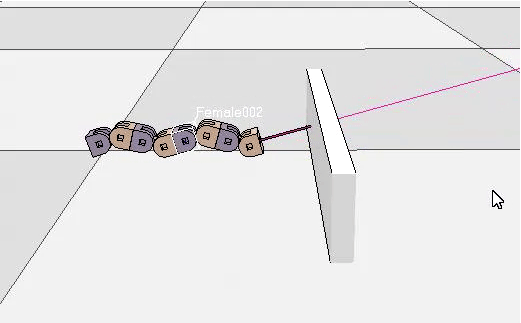
\includegraphics[scale=0.45]{detect.png}
	\end{itemize}
\end{frame}

\section{Task Accomplised}
\begin{frame}{Task Accomplised}
\begin{itemize}
		\item \textbf{Code and Documentation}
		    \begin{itemize}
		    \item Uploaded well-commented code (Arduino + Simulations) on GitHub for every stage.
		    \item Maintaining a detailed documentation of every step we take on GitHub Wiki of our repository.
            \end{itemize}
            
        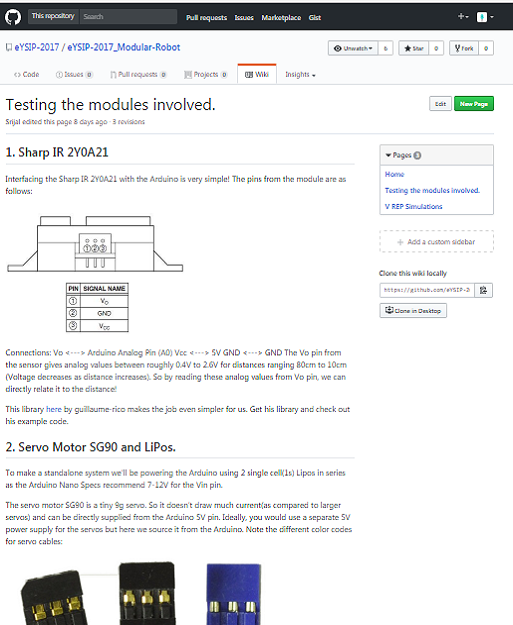
\includegraphics[scale=0.3]{1.png}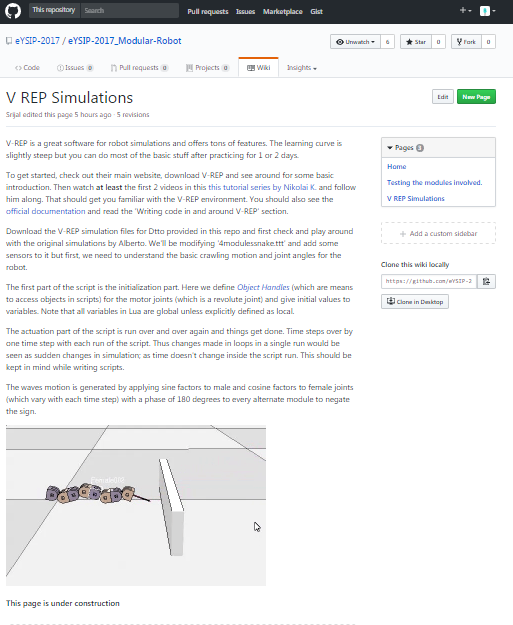
\includegraphics[scale=0.3]{2.png}
            
\end{itemize}
\end{frame}		


\section{Challenges Faced}
\begin{frame}{Challenges Faced}
	\begin{itemize}
		\item Appropriate screws (M1.7x4mm Flathead) were unavailable, so the CAD design was modified multiple times and the printing and assembling of modules has been delayed. \linebreak
		\item The specified Servo motor, MG92B is unavailable in local and online stores so we're forced to use a lower torque motor MG90S, which is the closest that can be fit under the given module dimensions.
 
	\end{itemize}
\end{frame}

\section{Future Plans}
\begin{frame}{Future Plans}
	\begin{itemize}
		\item All printed parts assembled. Four Robotic modules to be assembled.
		
		\item Develop effective and generalized algorithms for different motions.
		
		\item  Obstacle detection using sensors and decision making to avoid/overcome the obstacle while robot moves from one point to another.

	\end{itemize}
\end{frame}


\section{Thank You}
\begin{frame}{Thank You}
	\centering\LARGE Thank You !
\end{frame}
\end{document}
